\PassOptionsToPackage{unicode}{hyperref}
\documentclass[t]{beamer}

\usepackage[
  orientation=portrait,
  size=a0,
  scale=1.0,
]{beamerposter}

\usetheme{tudoposter}

\usepackage{fontspec}

\usepackage{polyglossia}
\setmainlanguage{german}

\usepackage{csquotes}
\usepackage{microtype}
\usepackage{mathtools}

\usepackage[
  math-style=ISO,
  bold-style=ISO,
  nabla=upright,
  partial=upright,
]{unicode-math}
\setmathfont{Tex Gyre Pagella Math}

\usepackage[locale=DE, binary-units]{siunitx}

\usepackage{blindtext}

\usepackage{multicol}
\setlength{\columnsep}{1em}

\usepackage{graphicx}
\usepackage{ragged2e}

\usepackage{tikz}

%% this is used to create an inline bibliography
\usepackage[backend=biber, style=numeric]{biblatex}
\addbibresource{biblatex-phys.bib}

\DeclareFieldFormat*{title}{\textit{#1}}
\renewcommand*{\bibfont}{\footnotesize}
\defbibenvironment{bibliography}
  {\noindent}
  {\unspace}
  {}

\renewbibmacro*{begentry}{%
  \usebeamercolor{bibliography item}%
  \color{bibliography item.fg}%
  \printtext[labelnumberwidth]{%
    \printfield{prefixnumber}%
    \printfield{labelnumber}%
  }%
  \setunit{\addnbspace}%
}
\renewcommand*{\finentrypunct}{\addperiod\space}

\newlength{\thirdtextwidth}
\setlength\thirdtextwidth{0.333333\textwidth}


\title{Datenanalyse mit IceCube Monte Carlo Daten}
\author{Maximilian Nöthe \and Kai Brügge}

\titlegraphic{%
  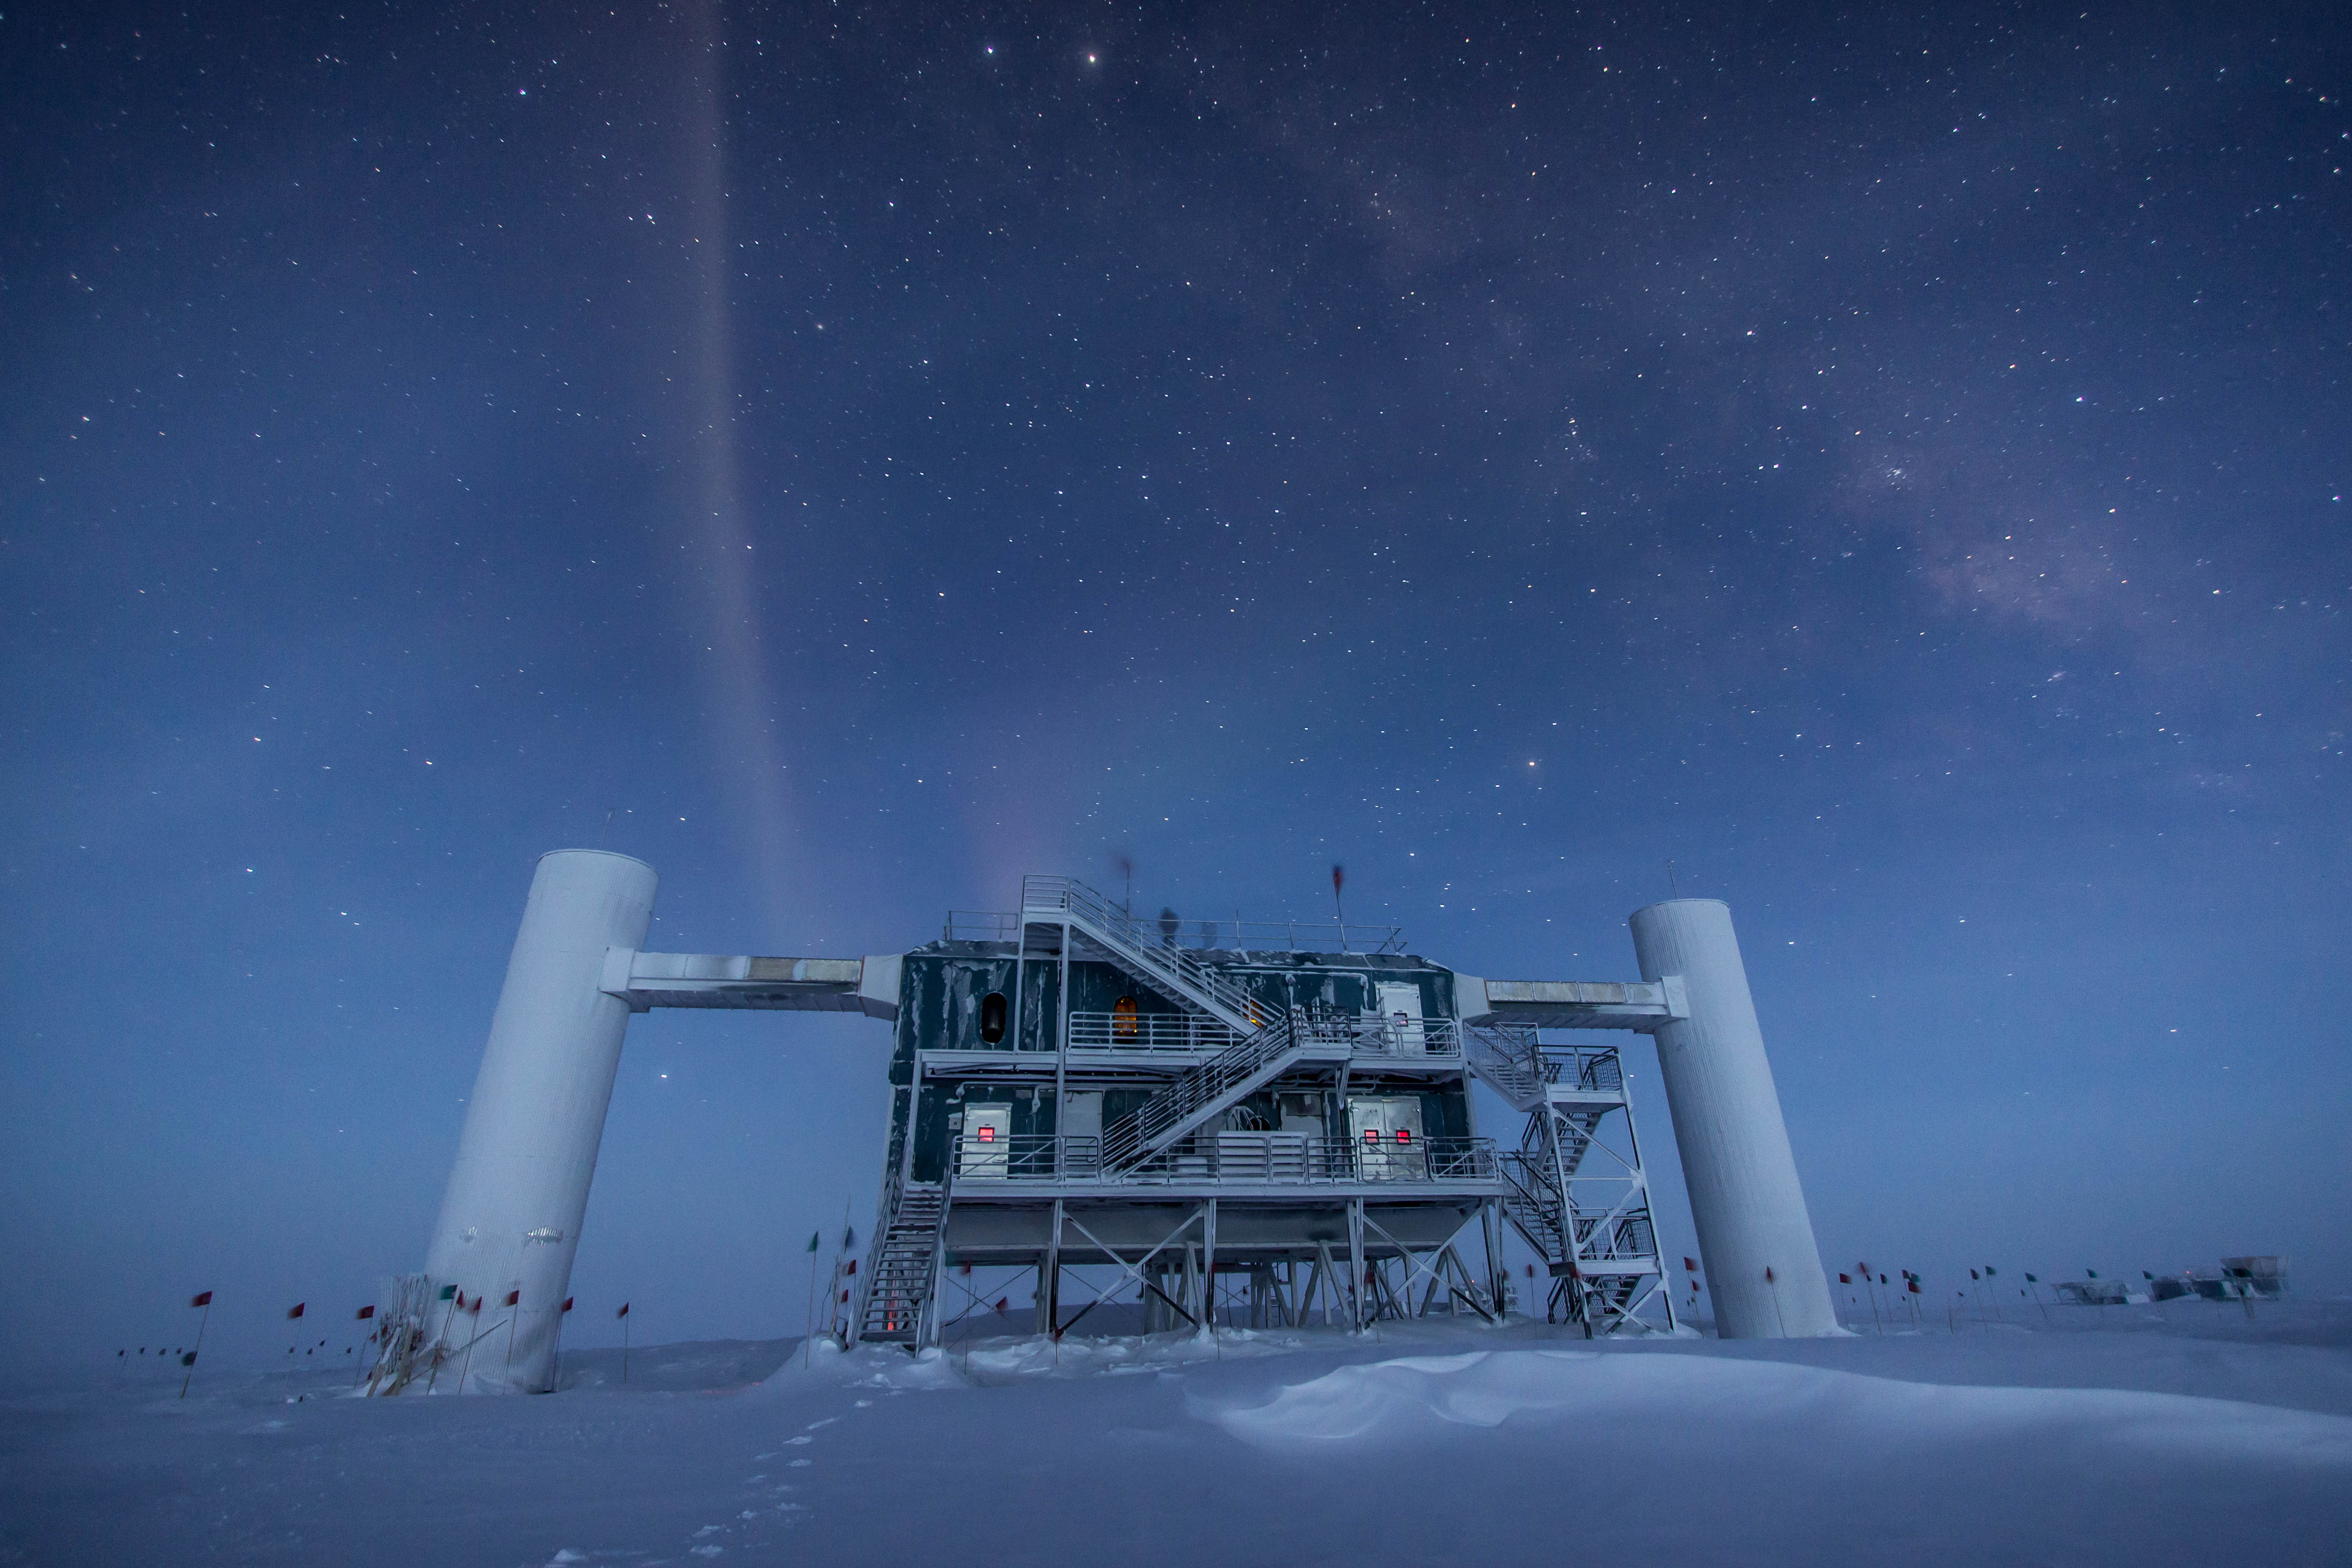
\includegraphics[width=\linewidth]{images/icecube.jpg}
}
\institute{%
  
\includegraphics[width=0.9\linewidth]{tudo.pdf}%
}

\begin{document}
  \begin{columns}[onlytextwidth]%
    \begin{column}{0.5\textwidth}%
      \begin{block}[equal height group=A]{Das IceCube Experiment}%
        \begin{columns}[onlytextwidth]%
          \begin{column}{0.48\textwidth}%
            \begin{figure}
              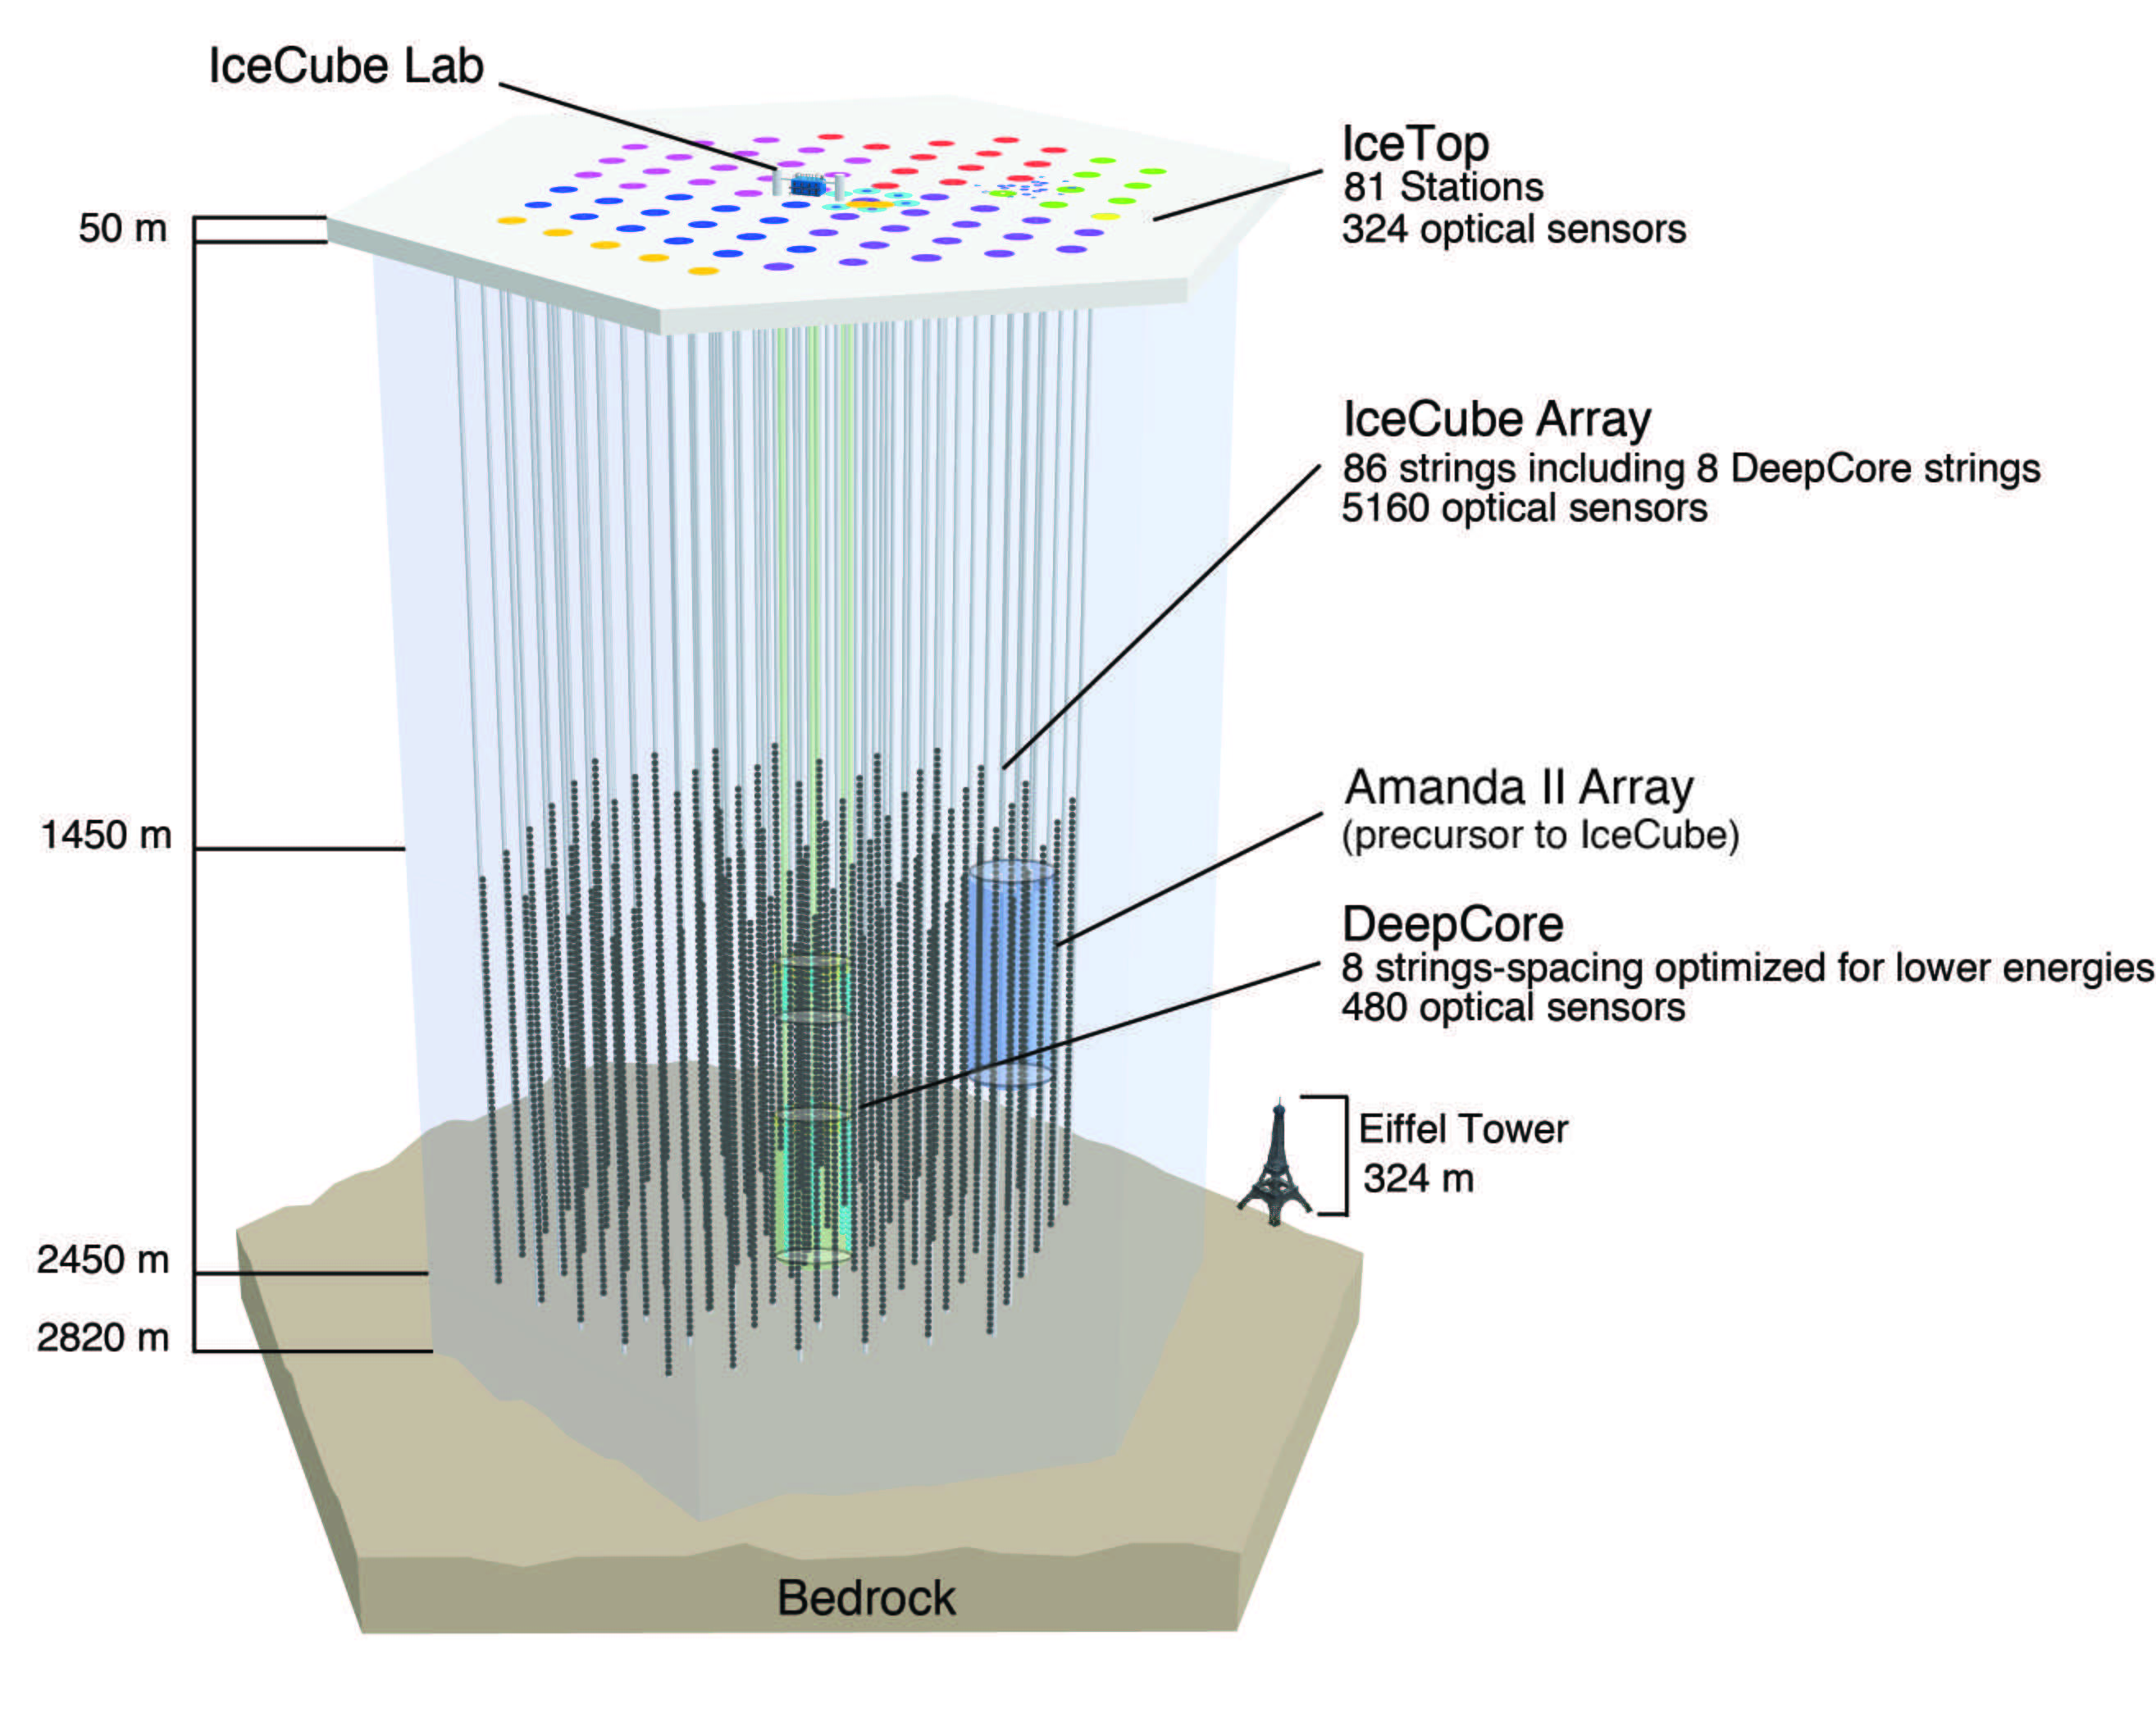
\includegraphics[width=\linewidth]{images/icecube_schema.jpg}\\
              \caption{Schematische Übersicht des IceCube Detektors.}
            \end{figure}
          \end{column}\hfill
          \begin{column}{0.48\textwidth}%
            \justifying
            Das IceCube Experiment befindent sich im Eis des geographischen Südpols.
            Das Ziel des Experiments ist das Messen von kosmischen Neutrinos.
            Hierbei stellt ein Untergrund aus atmosphärischen Myonen und Neutrinos eine
            große Herausforderung dar.

            Nachgewiesen werden Neutrinos über das Tscherenkow-Licht von Sekundärteilchen,
            die bei der Wechselwirkung der Neutrinos mit den Atomen des Eises entstehen.

            Der Detektor besteht aus insgesamt \num{5160} Photodetektoren,
            die an \num{86} einzelnen Strängen in einer Tiefe zwischen
            \SI{1450}{\meter} und \SI{2450}{\meter} im Eis eingelassen sind.

            IceCube nimmt pro Tag etwa \SI{1}{\tera\byte} Daten. 
            Der erste Nachweis kosmischer Neutrinos gelang 2013.
          \end{column}%
        \end{columns}%
      \end{block}%
    \end{column}%
    \begin{column}{0.5\textwidth}%
      \begin{block}[equal height group=A]{Dataming}%
        \begin{multicols}{2}
          Das sehr kleine Signal-zu-Untergrund-Verhältnis von ca.\ $1:10^6$ und die 
          riesigen Datenmengen des IceCube Exeperiments machen das 
          verwenden von Verfahren des maschinellen Lernens bzw. Data Minings nötig, 
          um Signal-Ereignisse aus den Daten zu extrahieren.

          In diesem Versuch wird die Leistungsfähigkeit verschiedener Verfahren
          des maschinellen Lernens auf simulierten Daten des IceCube Experiments 
          zur Klassifizierung in Signal bzw. Untergrund evaluiert.

          Signal sind hierbei alle Neutrino-Ereignisse, Untergrund sind hauptsächlich
          atmosphärische Myonen.

          Verwendet werden Methoded des überwachten maschinellen Lernens.
          Überwachte Lerner müssen auf einem Datensatzt mit bekannten Wahrheiten
          \enquote{trainiert} werden und können dann auf Daten mit unbekannter 
          Wahrheit angewendet werden.

          Von großer Wichtigkeit ist die Validierung der Performanz des Modells.
          Hierzu wird eine Kreuzvalidierung verwendet und mehrere Leistungskennzahlen
          ausgewertet.
        \end{multicols}
      \end{block}%
    \end{column}%
  \end{columns}%

  \begin{columns}[onlytextwidth]%
    \begin{column}{0.5\textwidth}%
      \begin{block}[equal height group=B]{Verwendete Software}%
        Für den Versuch wird der sogenannte \enquote{Scientific Python Stack} verwendent.\par
        \begin{tikzpicture}
          \node at (0, 0) {
\includegraphics[height=3.5cm]{images/python.pdf}};
          \node at (-3cm, -6cm) {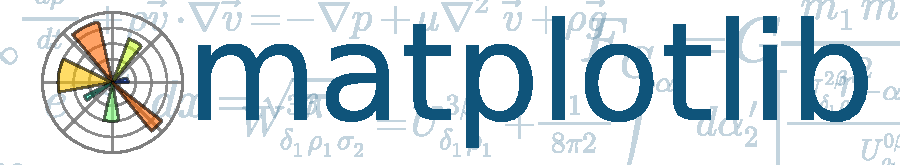
\includegraphics[height=2.5cm]{images/matplotlib.pdf}};
          \node at (10cm, -2cm) {
\includegraphics[height=4.5cm]{images/scikit-learn.pdf}};
        \end{tikzpicture}
      \end{block}
    \end{column}%
  \end{columns}%

  \vspace*{\fill}
  \begin{block}[equal height group=bottom, fonttitle=\normalsize]{Referenzen}
    \begin{multicols}{3}
      \nocite{*}\footnotesize%
      \printbibliography%
    \end{multicols}
  \end{block}
\end{document}
